\documentclass{article}
\usepackage{graphicx}
\usepackage{float}
\usepackage[margin=.75in]{geometry}

\usepackage{hyperref}
\hypersetup{
    colorlinks=true,
    linkcolor=blue,
    filecolor=magenta,      
    urlcolor=cyan,
}
 
\urlstyle{same}
\begin{document}

Code used in production of plots for this section can be found at https://github.com/cfmcginn/SystBio/tree/master/HW9.
\section{1.c+1.d}

\begin{figure}[H]
    \centering
    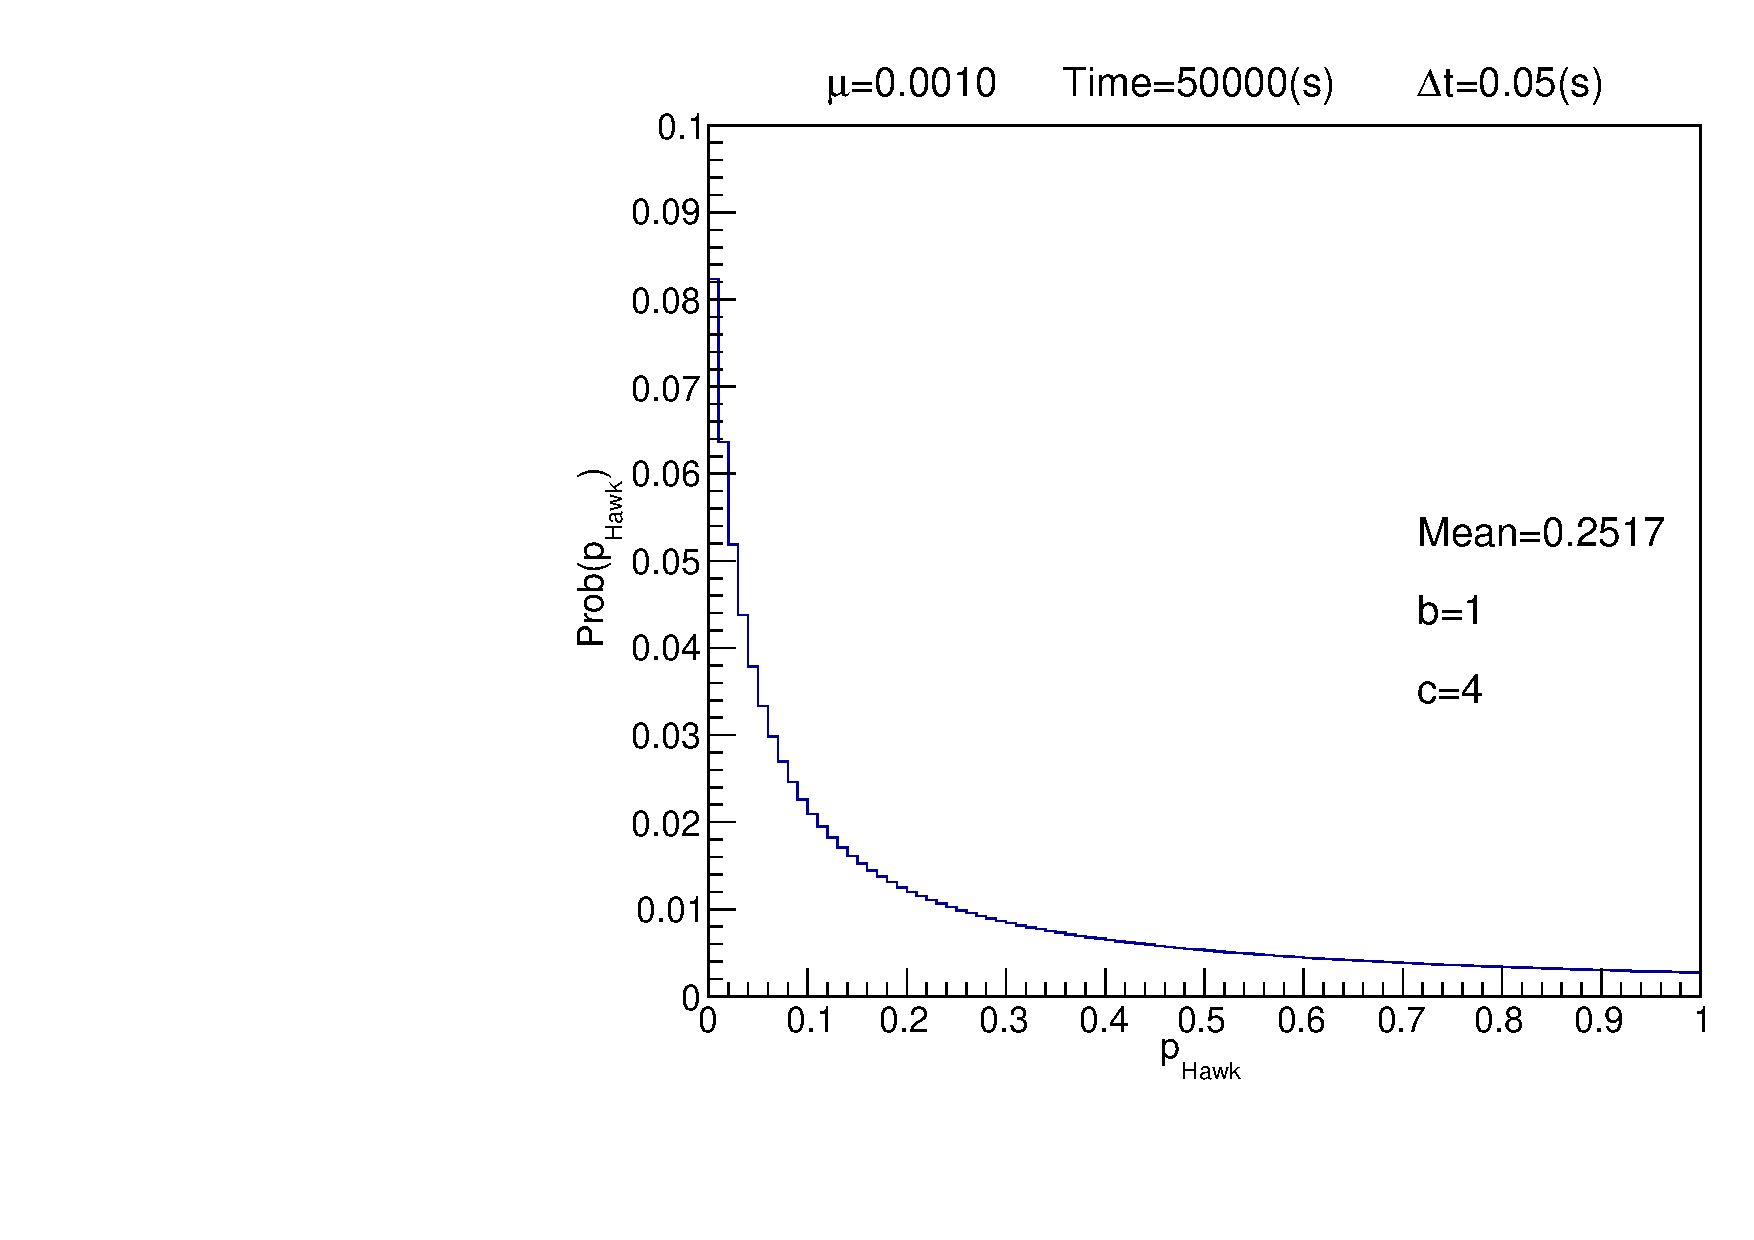
\includegraphics[width=.45\textwidth]{hawkDoveProb_Mu0p0010_20171201.pdf} 
    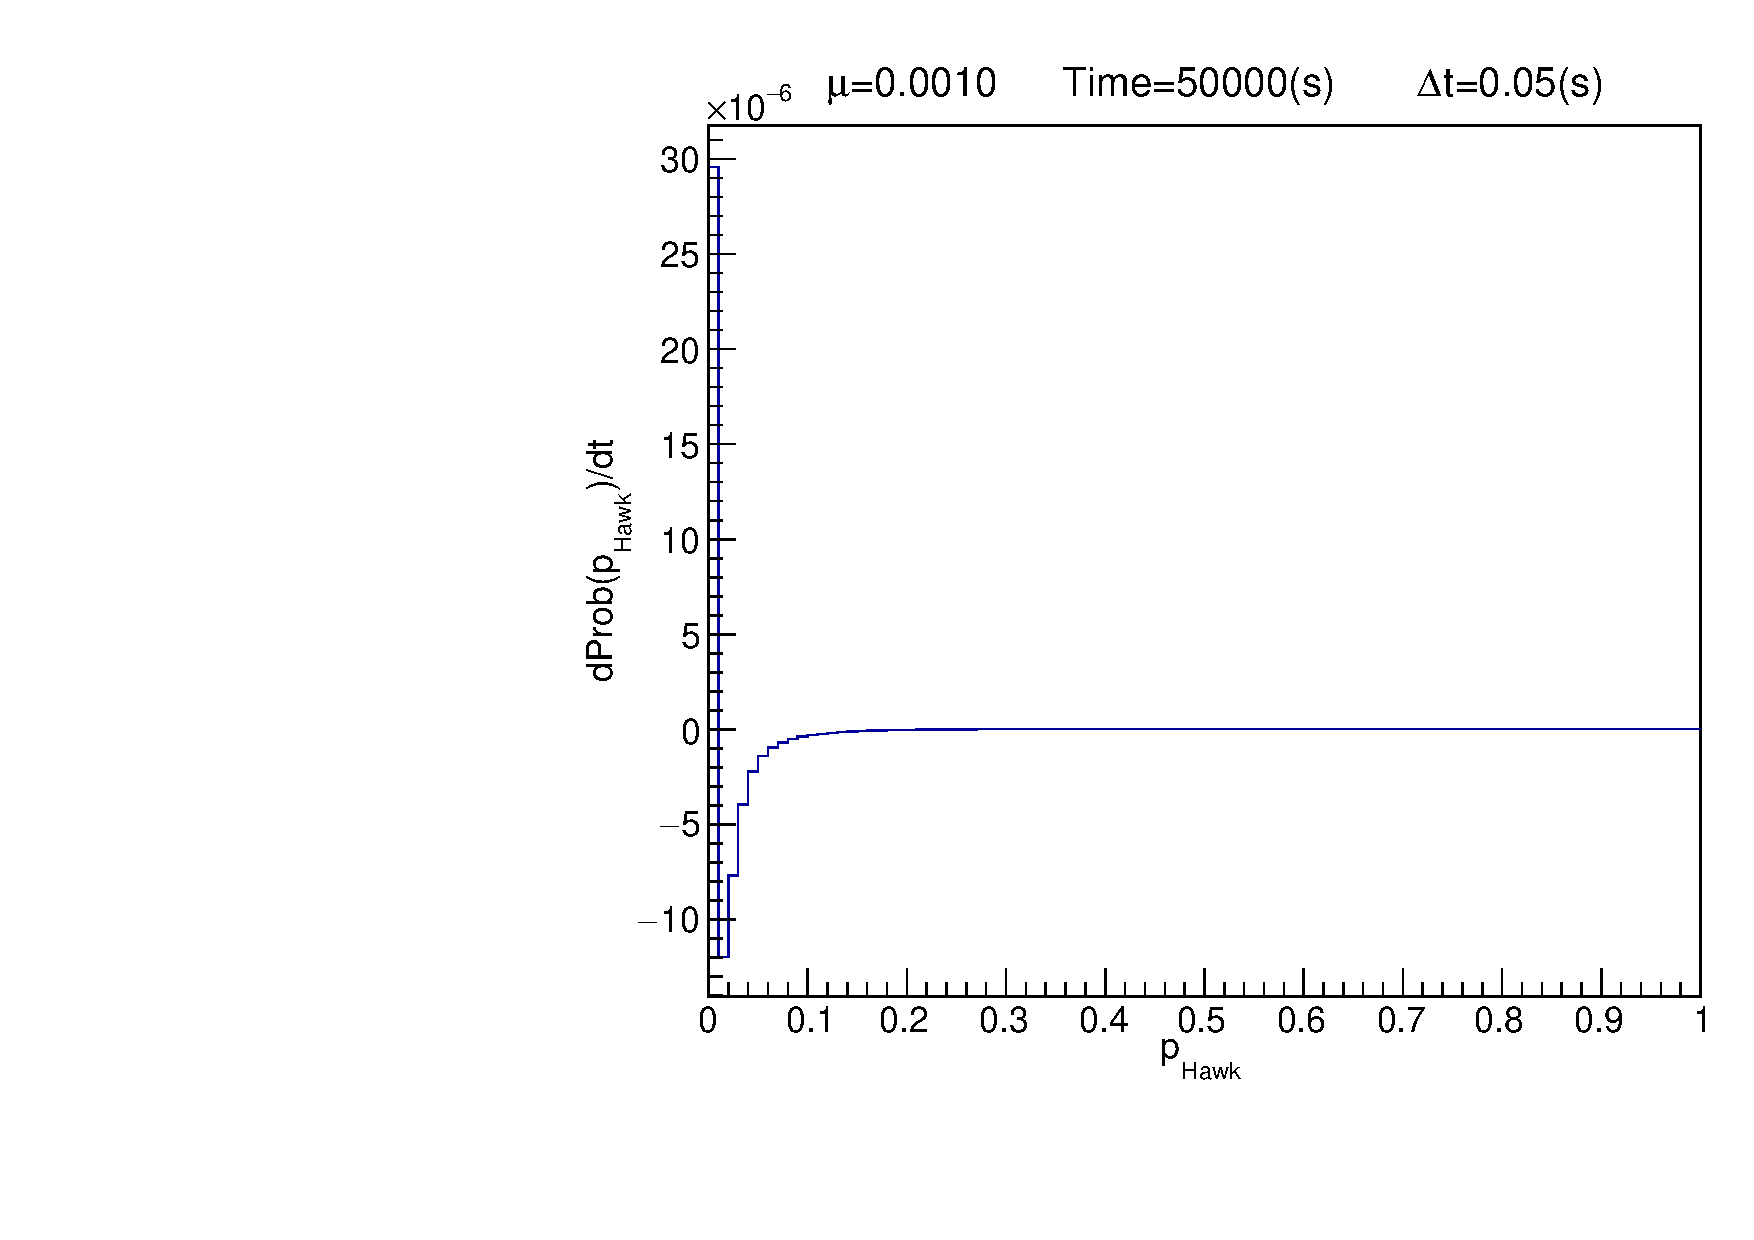
\includegraphics[width=.45\textwidth]{hawkDoveProb_DPDT_Mu0p0010_20171201.pdf} 
    \caption{}
    \label{fig:fig1}
\end{figure}

\begin{figure}[H]
    \centering
    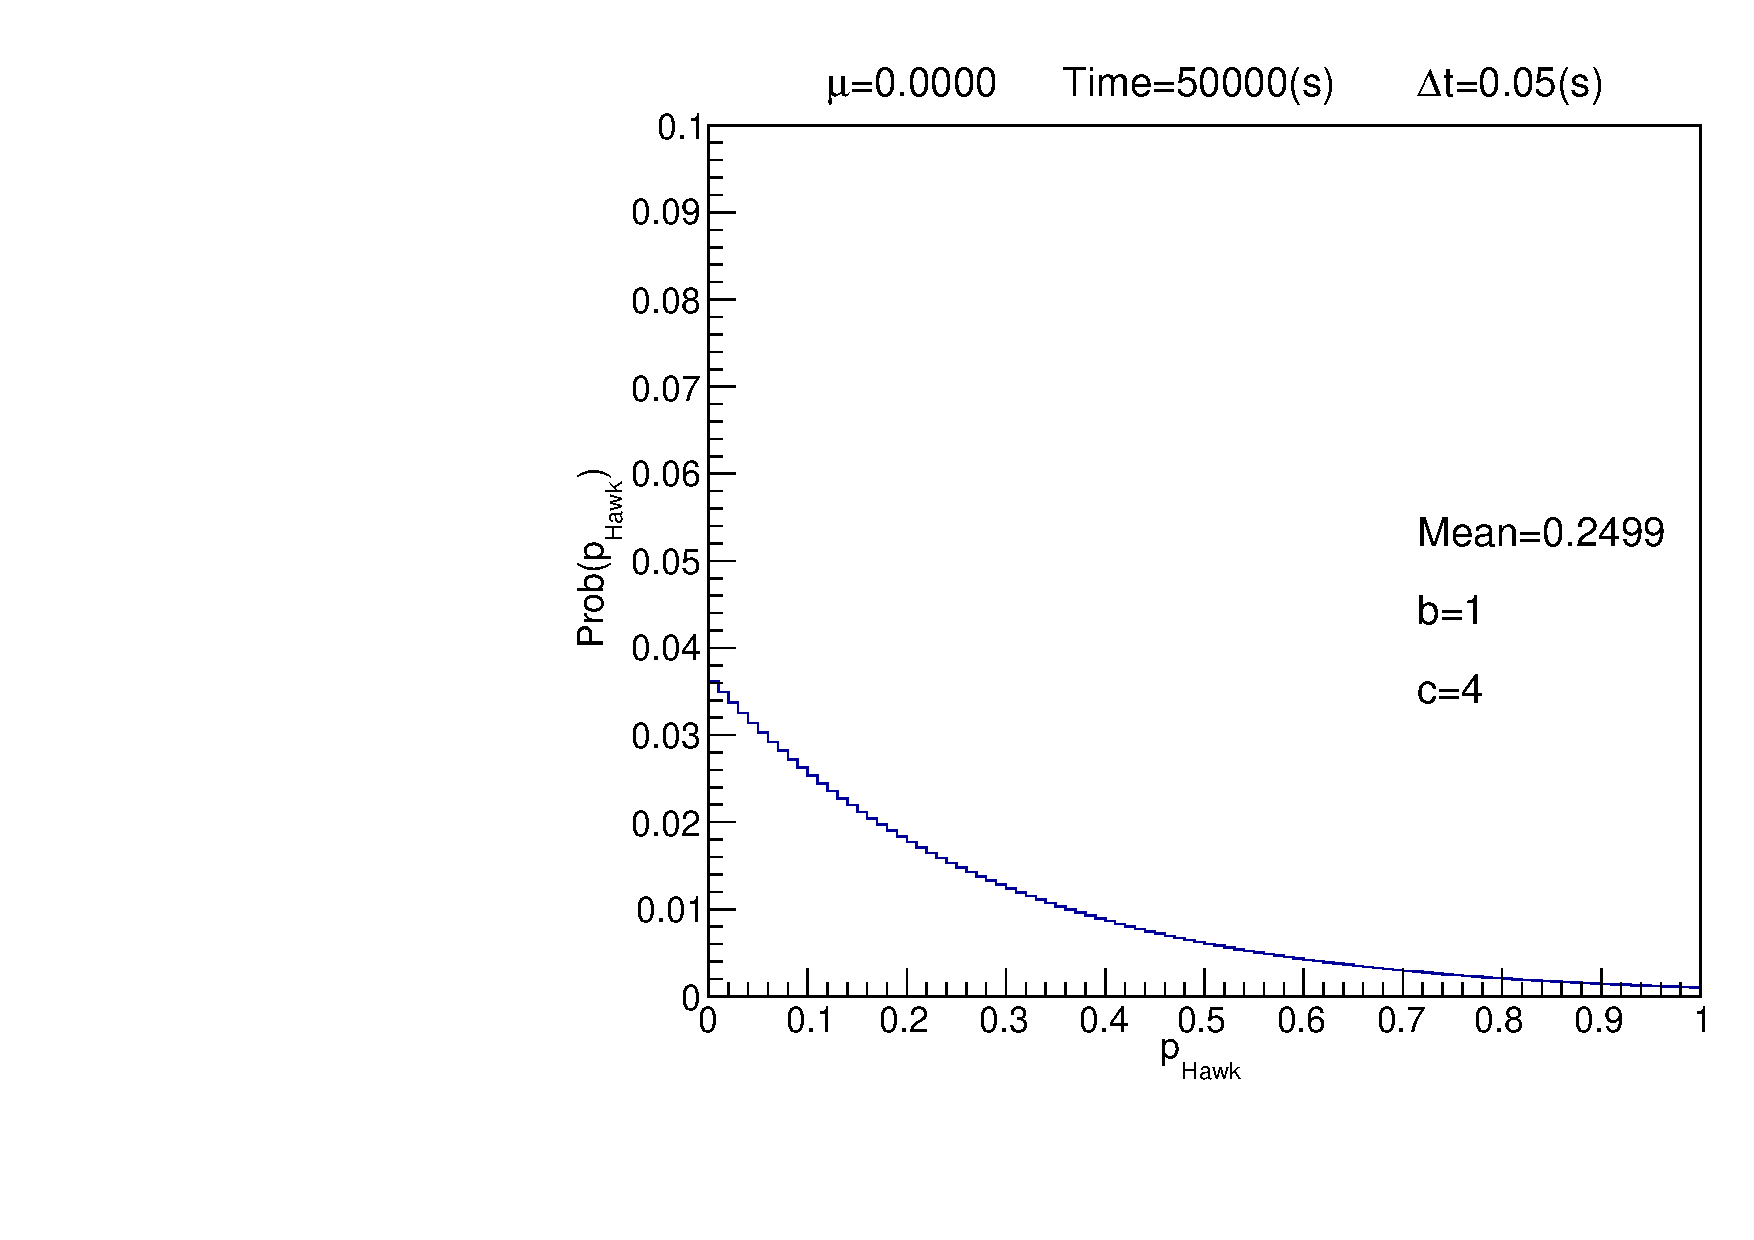
\includegraphics[width=.45\textwidth]{hawkDoveProb_Mu0p0000_20171201.pdf} 
    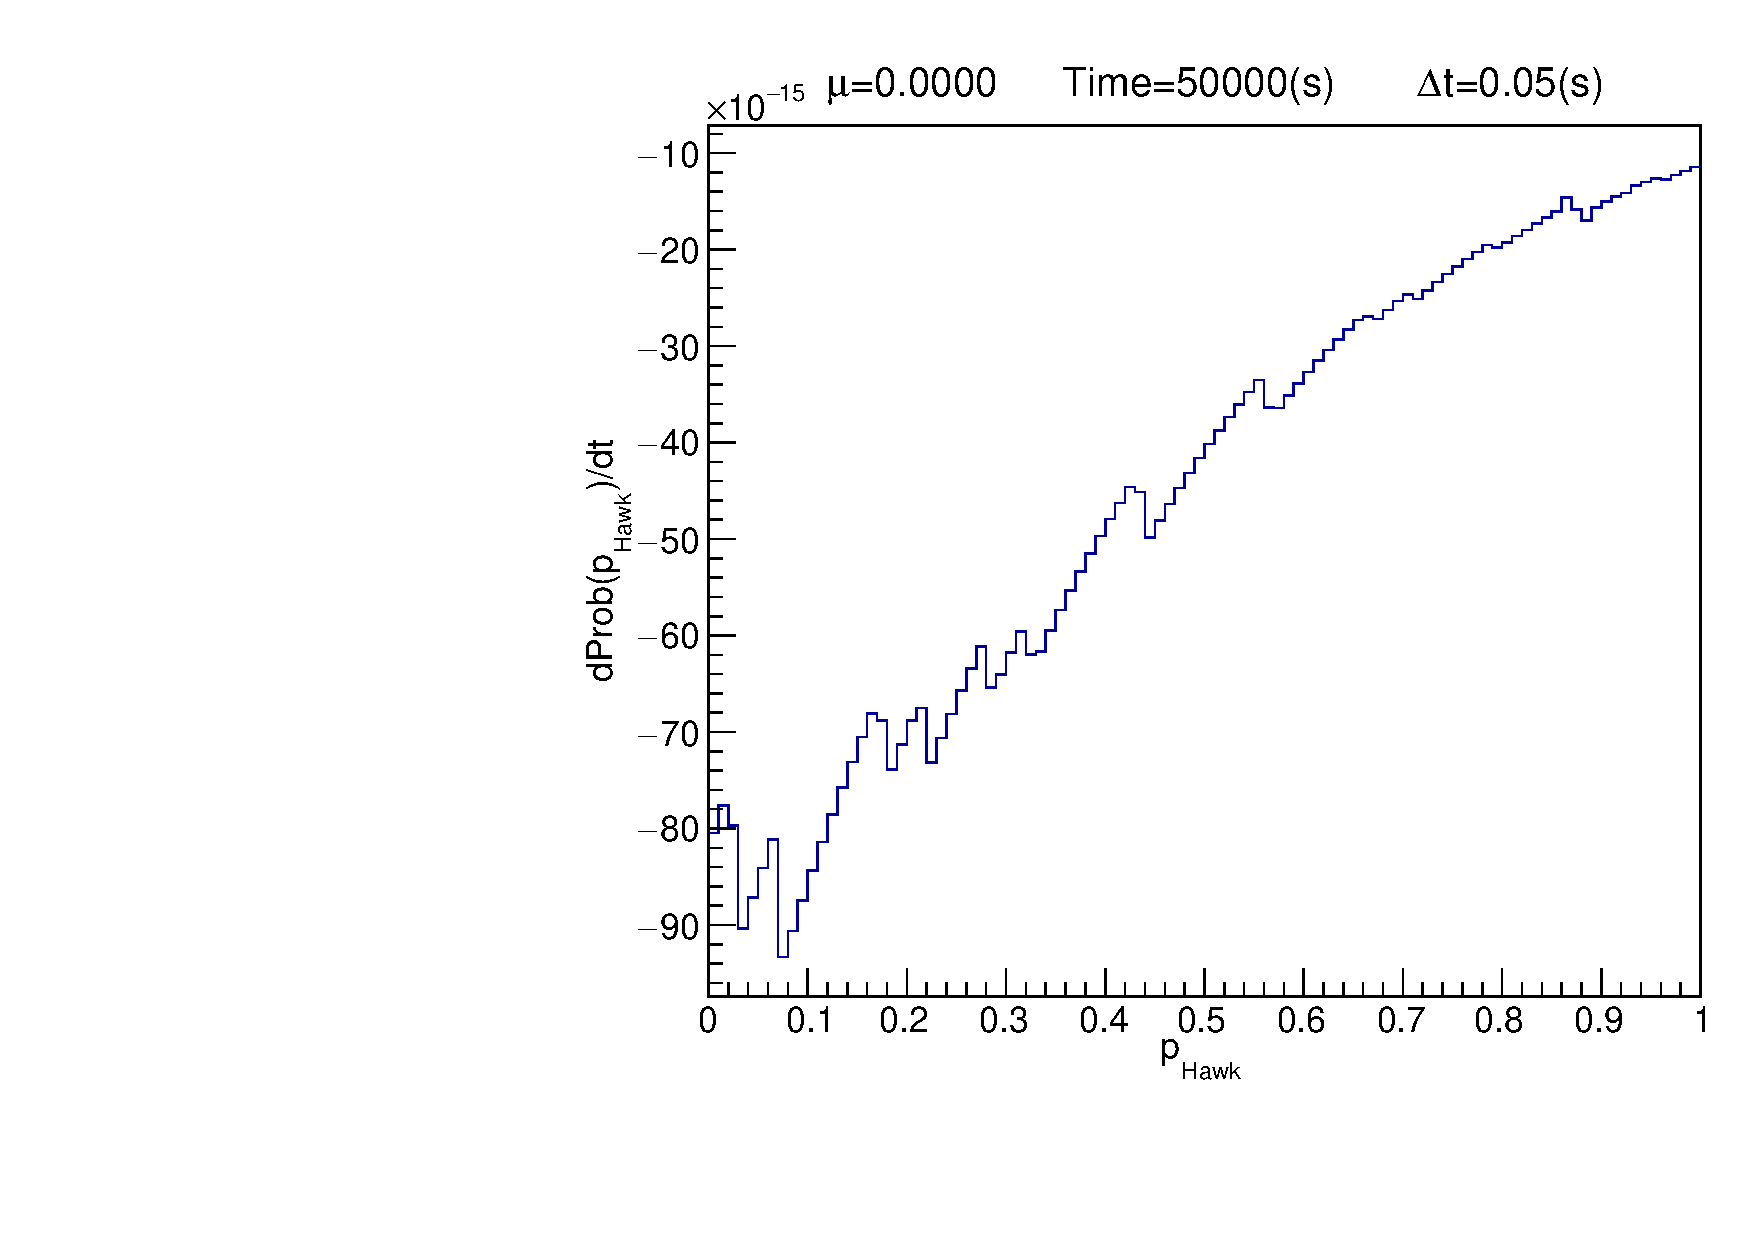
\includegraphics[width=.45\textwidth]{hawkDoveProb_DPDT_Mu0p0000_20171201.pdf} 
    \caption{}
    \label{fig:fig2}
\end{figure}

The mean is related to b and c parameters as the ratio of b over c. Thus with different dynamics we still see the same mean when checking the lefthand plots in Fig.~\ref{fig:fig1} and Fig.~\ref{fig:fig2}. These plots differ by mutation rate of 0.001 and 0.000. The impact of a flat mutation rate is to result in a long, flatter tail to larger hawk probability, and a sharper peak in the dove regime.

\section{2.d.1-4}

\begin{figure}[H]
    \centering
    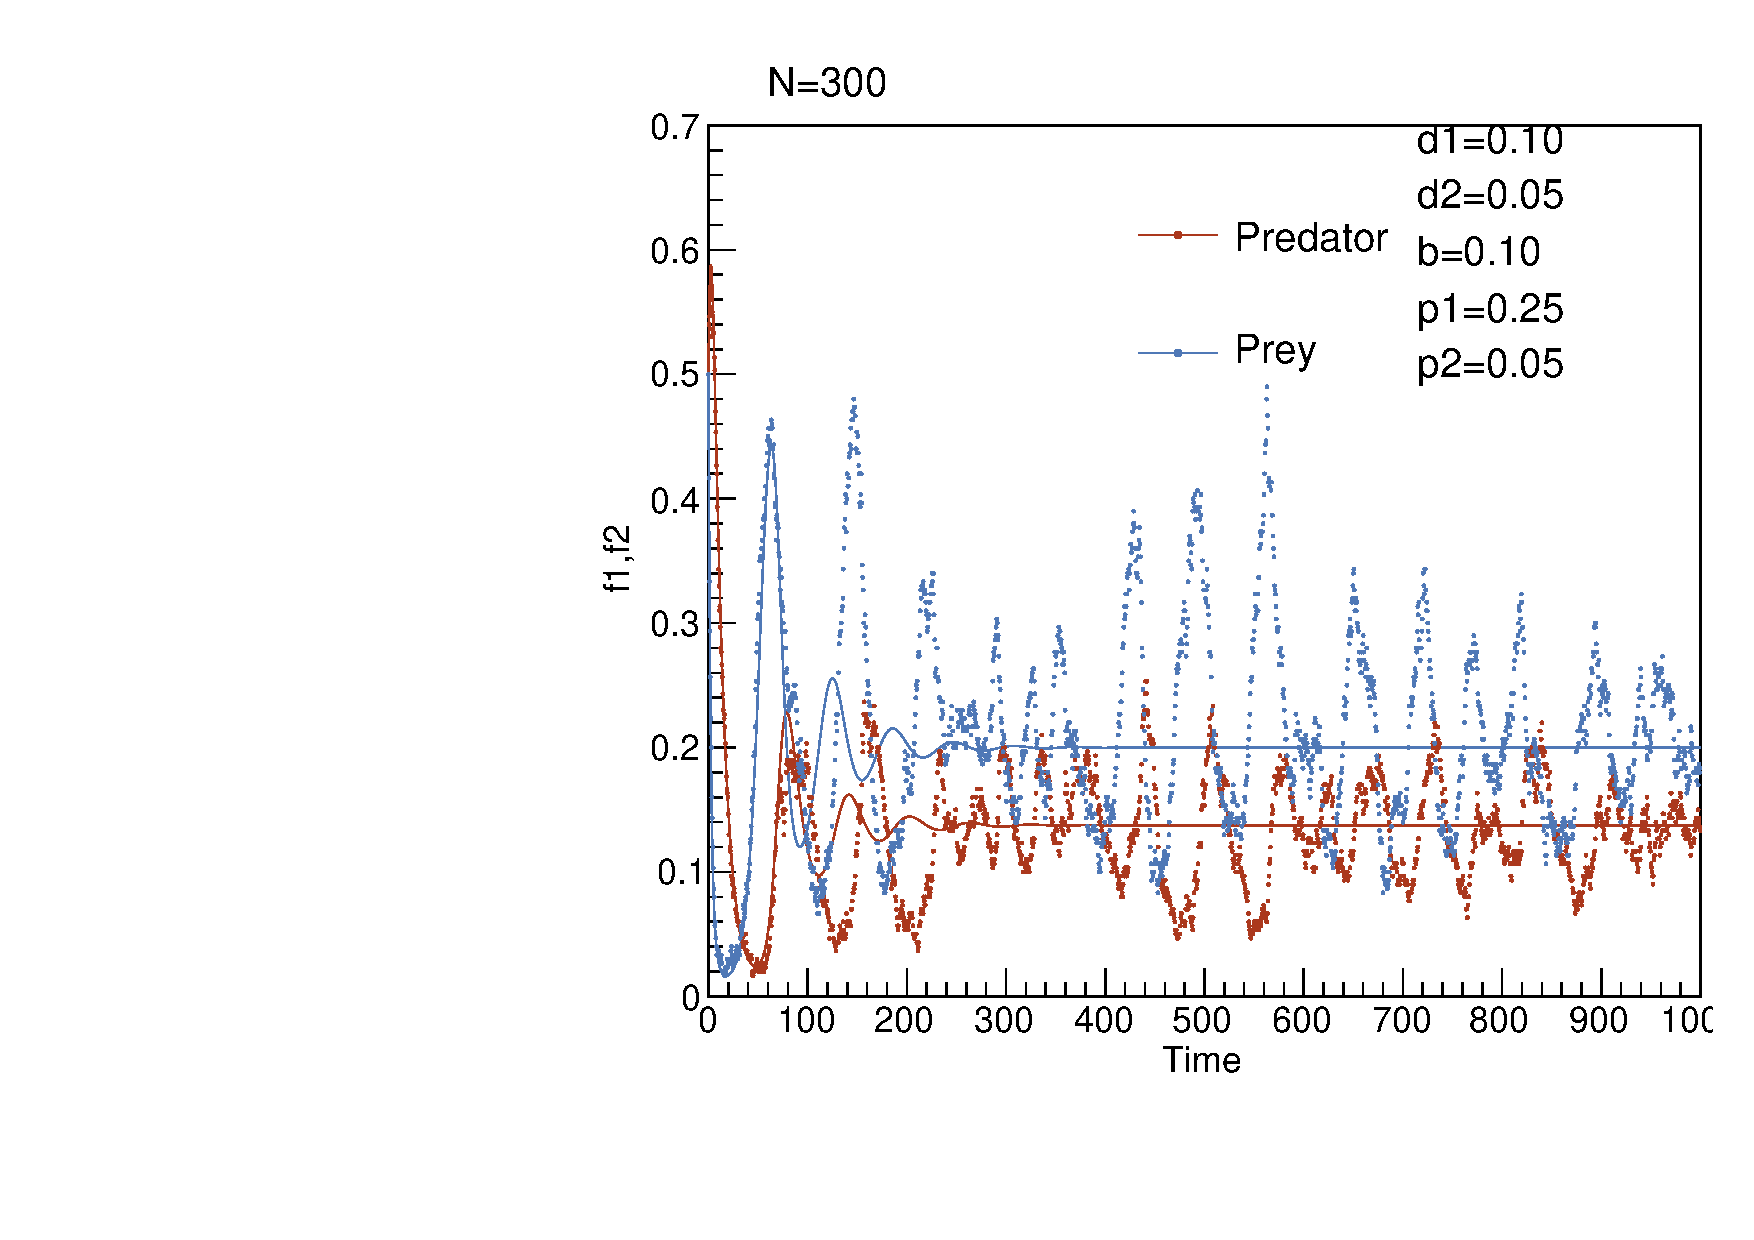
\includegraphics[width=.32\textwidth]{stochIBM_NTot300_p10p25_20171201.pdf} 
    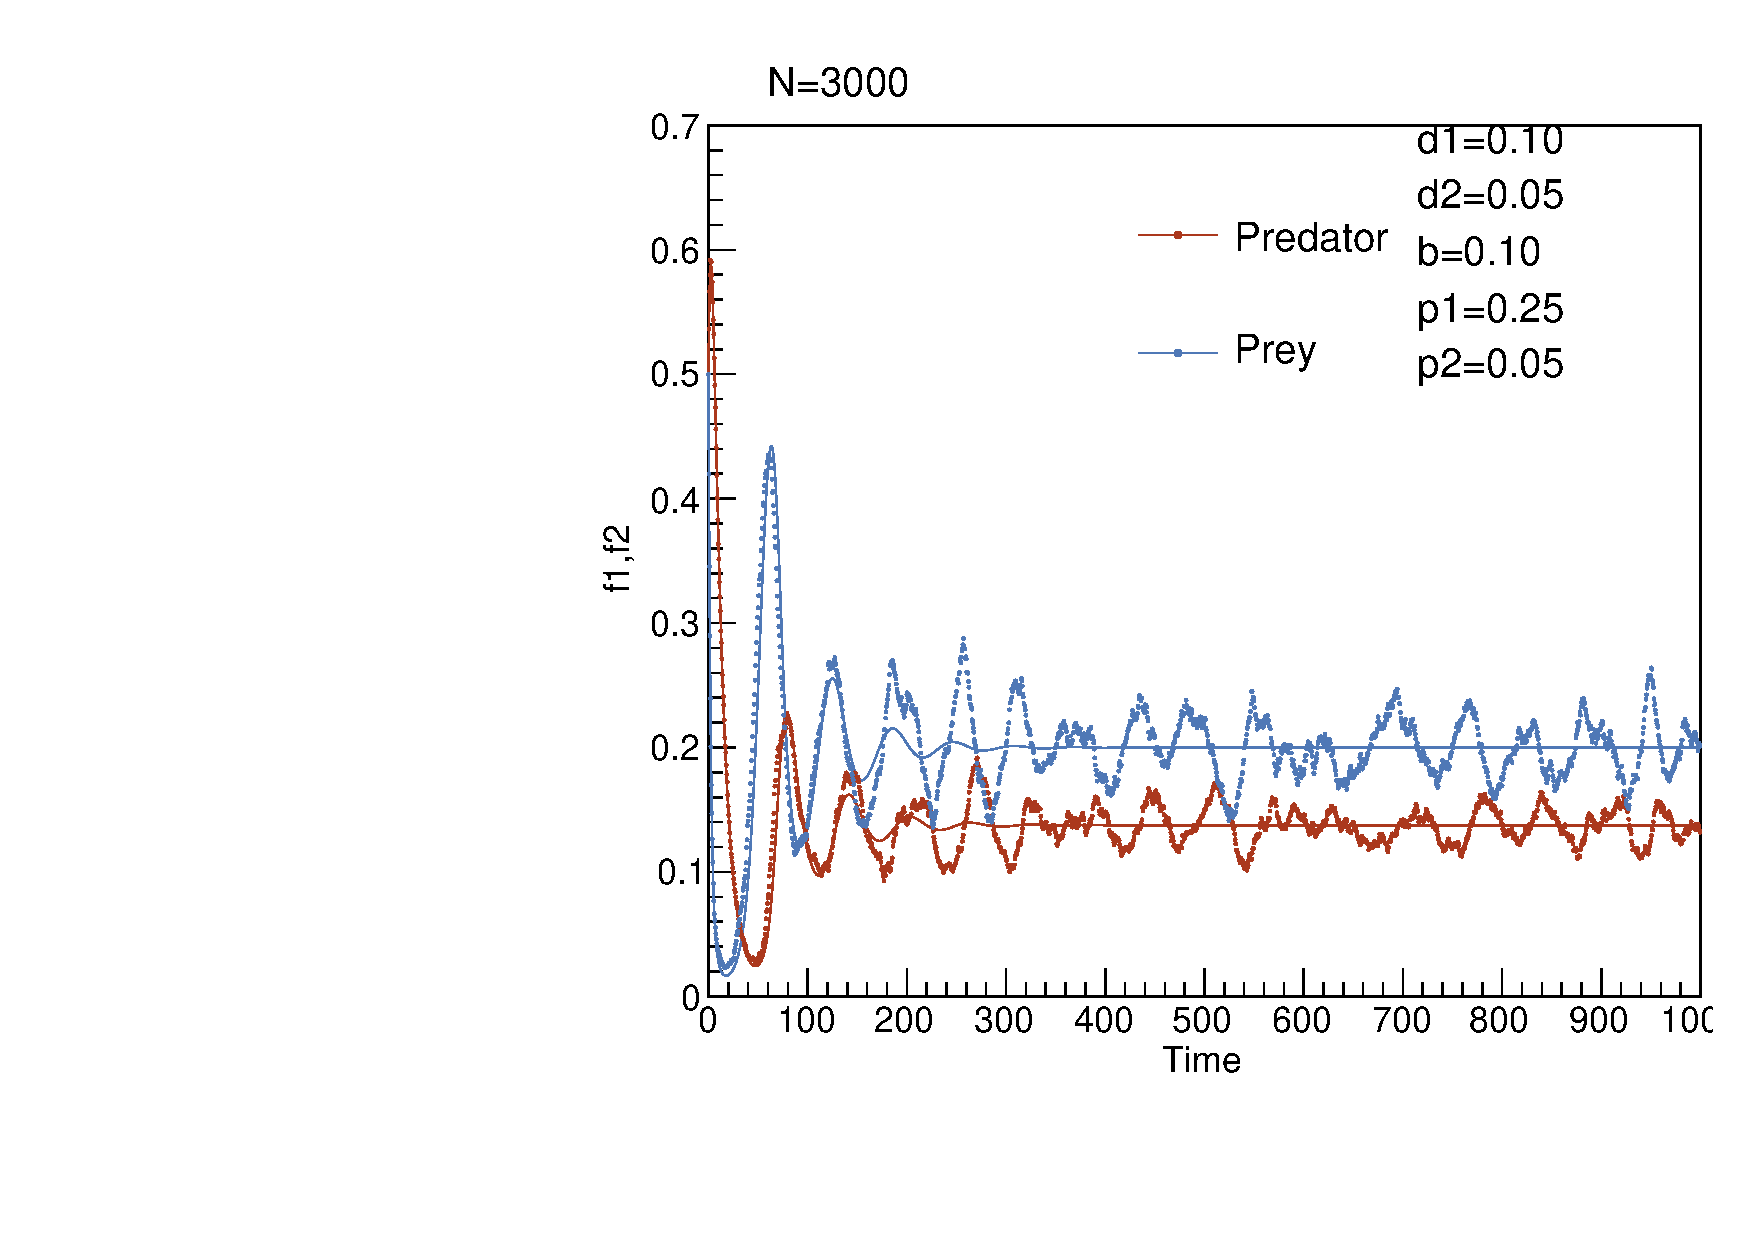
\includegraphics[width=.32\textwidth]{stochIBM_NTot3000_p10p25_20171201.pdf}  
    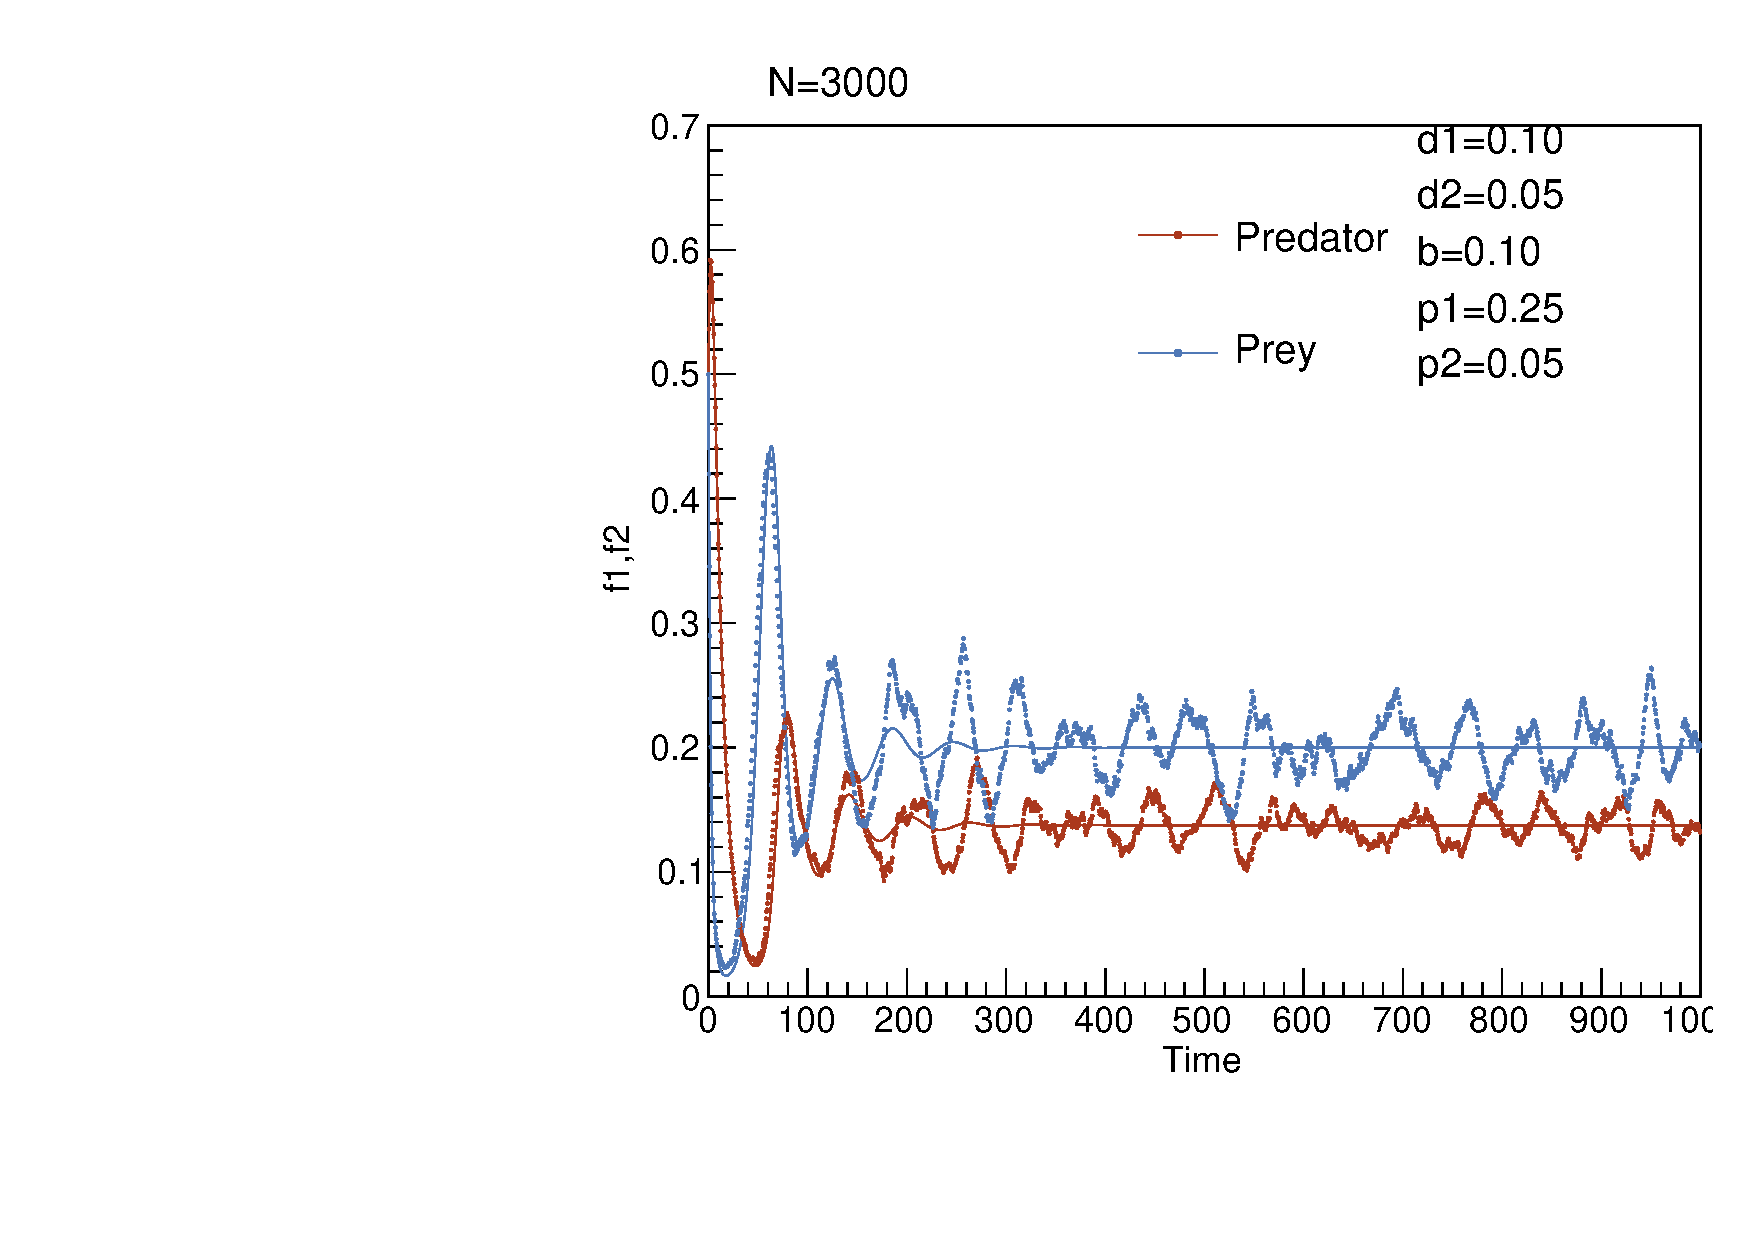
\includegraphics[width=.32\textwidth]{stochIBM_NTot3000_p10p25_20171201.pdf} 
    \caption{}
    \label{fig:fig3}
\end{figure}

In Fig.~\ref{fig:fig3} we see transient oscillations in the solid line (deterministic model) for the given set of parameters. The frequency of these oscillations will go as the square root of the absolute value of trace squared minus four times determinant. For the given set of parameters we get omega of ~.2. Overlaid on top of the deterministic model in Fig.~\ref{fig:fig3} is the Gillepsie simulation of the stochastic formula for three different population sizes N, going from left to right as 300, 3000, and 30000. While the deterministic model is identical in all three cases, the fluctuations of the stochastic model varies w/ the population size significantly.

\begin{figure}[H]
    \centering
    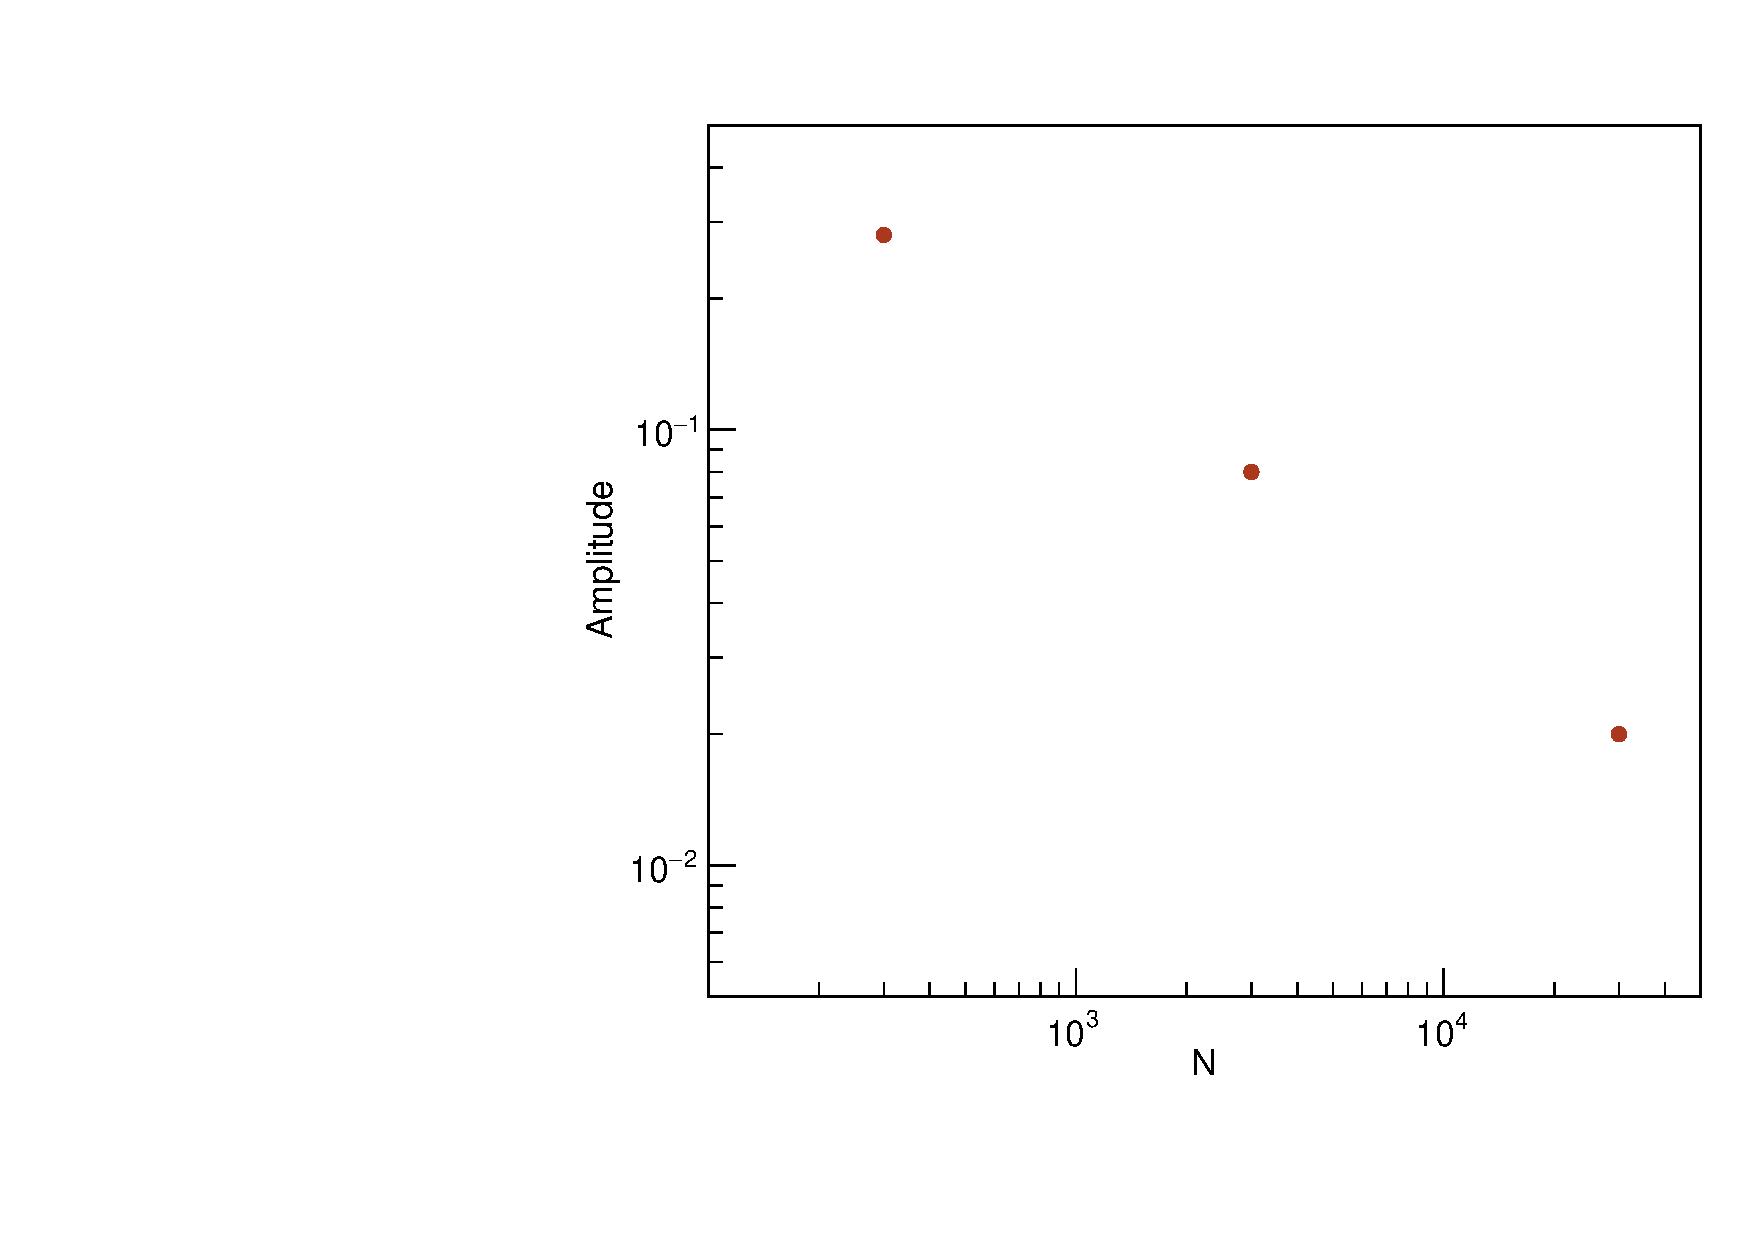
\includegraphics[width=.6\textwidth]{amplitude.pdf} 
    \caption{}
    \label{fig:fig3b}
\end{figure}

In Fig.~\ref{fig:fig3b} we have the amplitude of the stochastic oscillations as a function of the three N parameters (extracted roughly from the plots by eye. The slope is roughly -.5 on the log scale, which would mean a dependence on N of one over root N.

\begin{figure}[H]
    \centering
    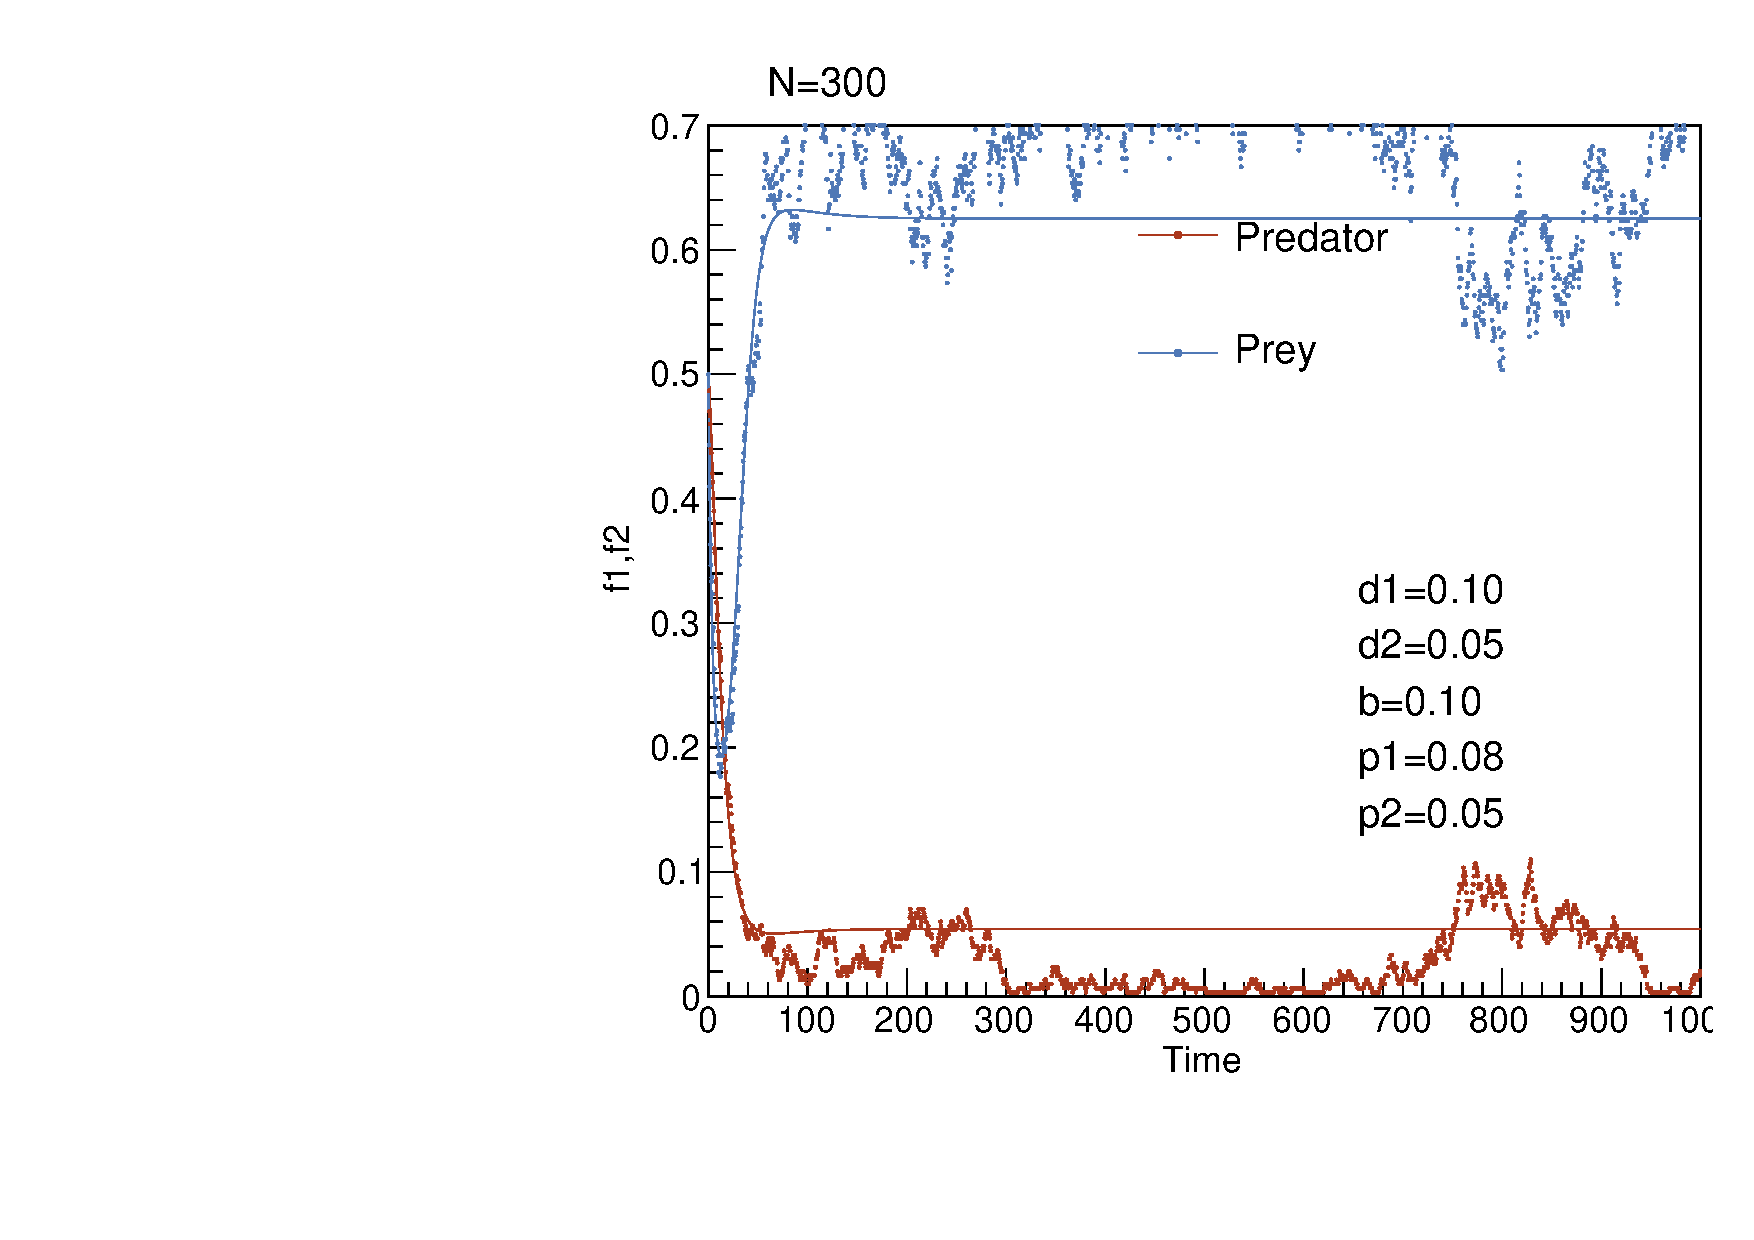
\includegraphics[width=.32\textwidth]{stochIBM_NTot300_p10p08_20171201.pdf} 
    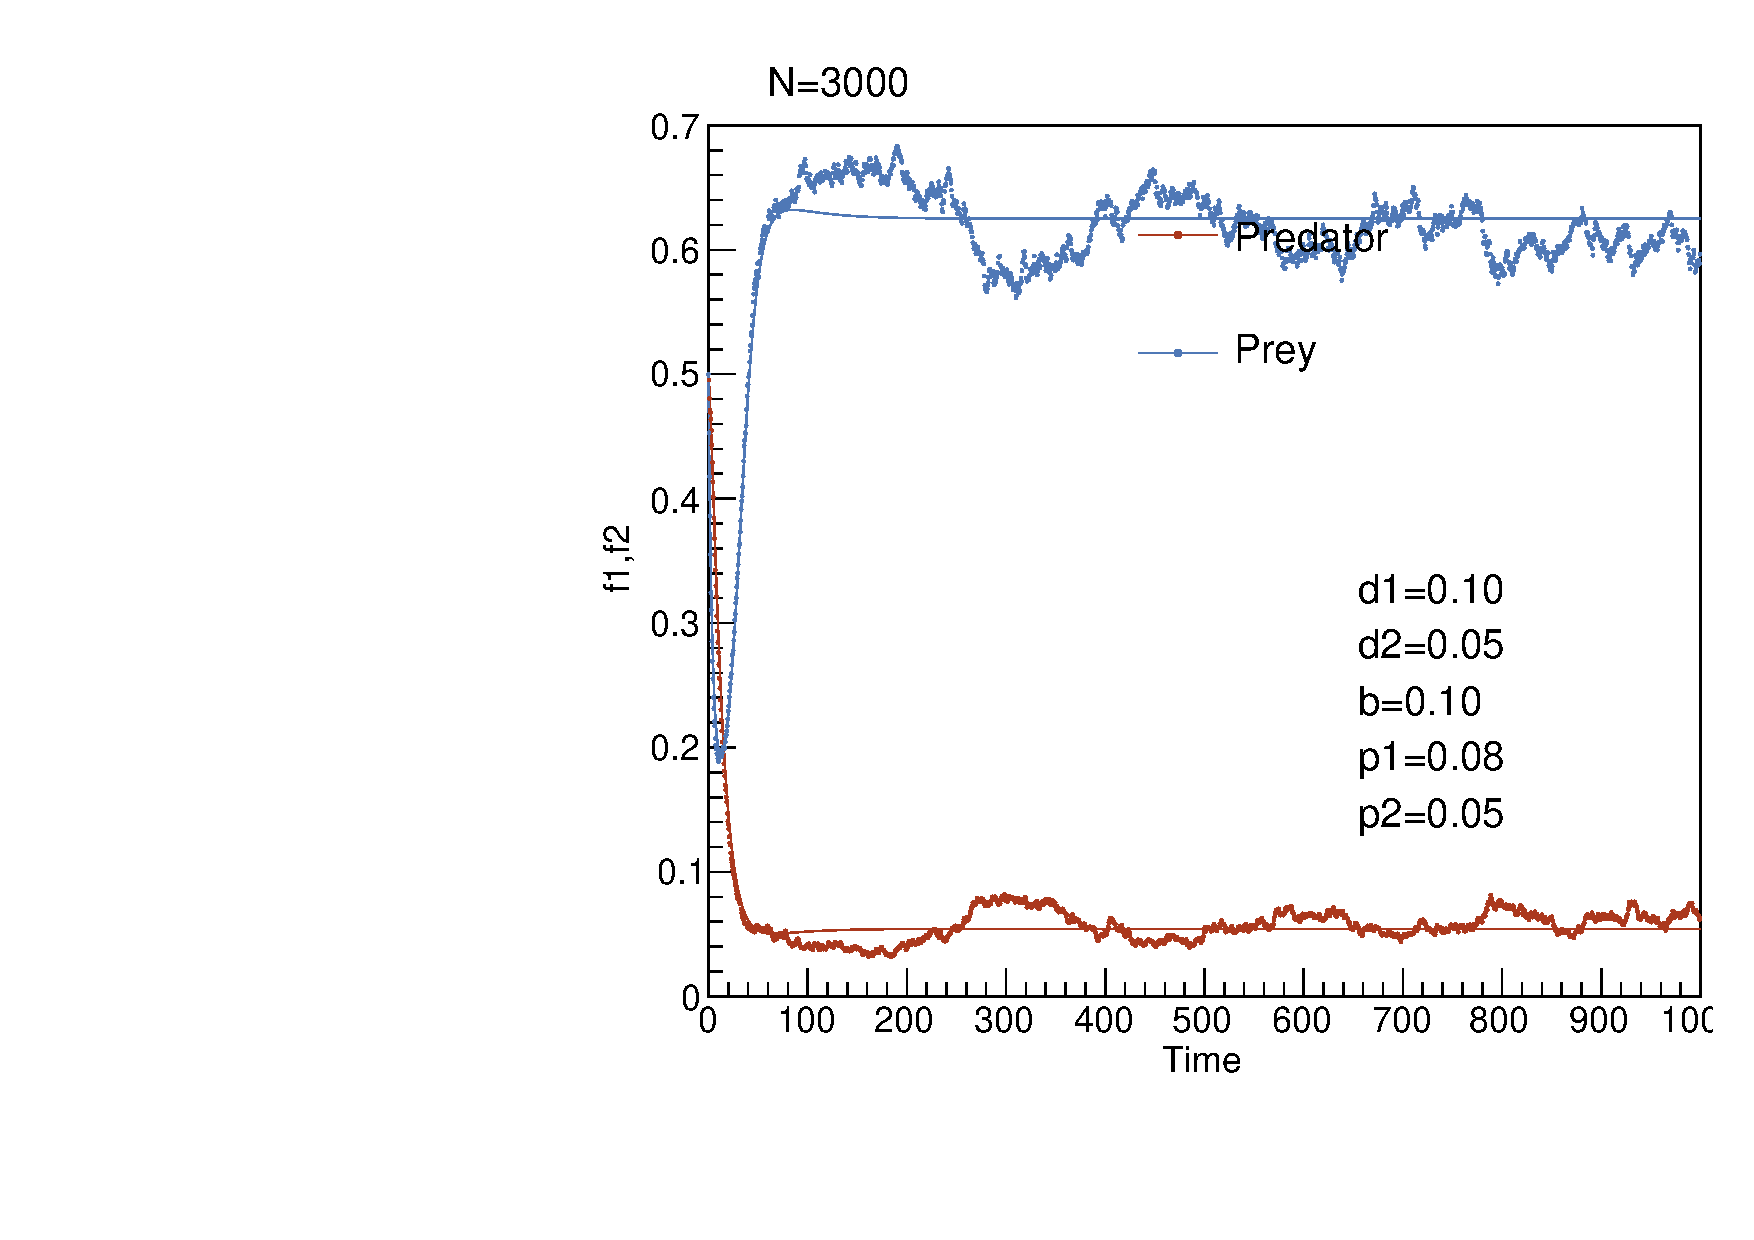
\includegraphics[width=.32\textwidth]{stochIBM_NTot3000_p10p08_20171201.pdf}  
    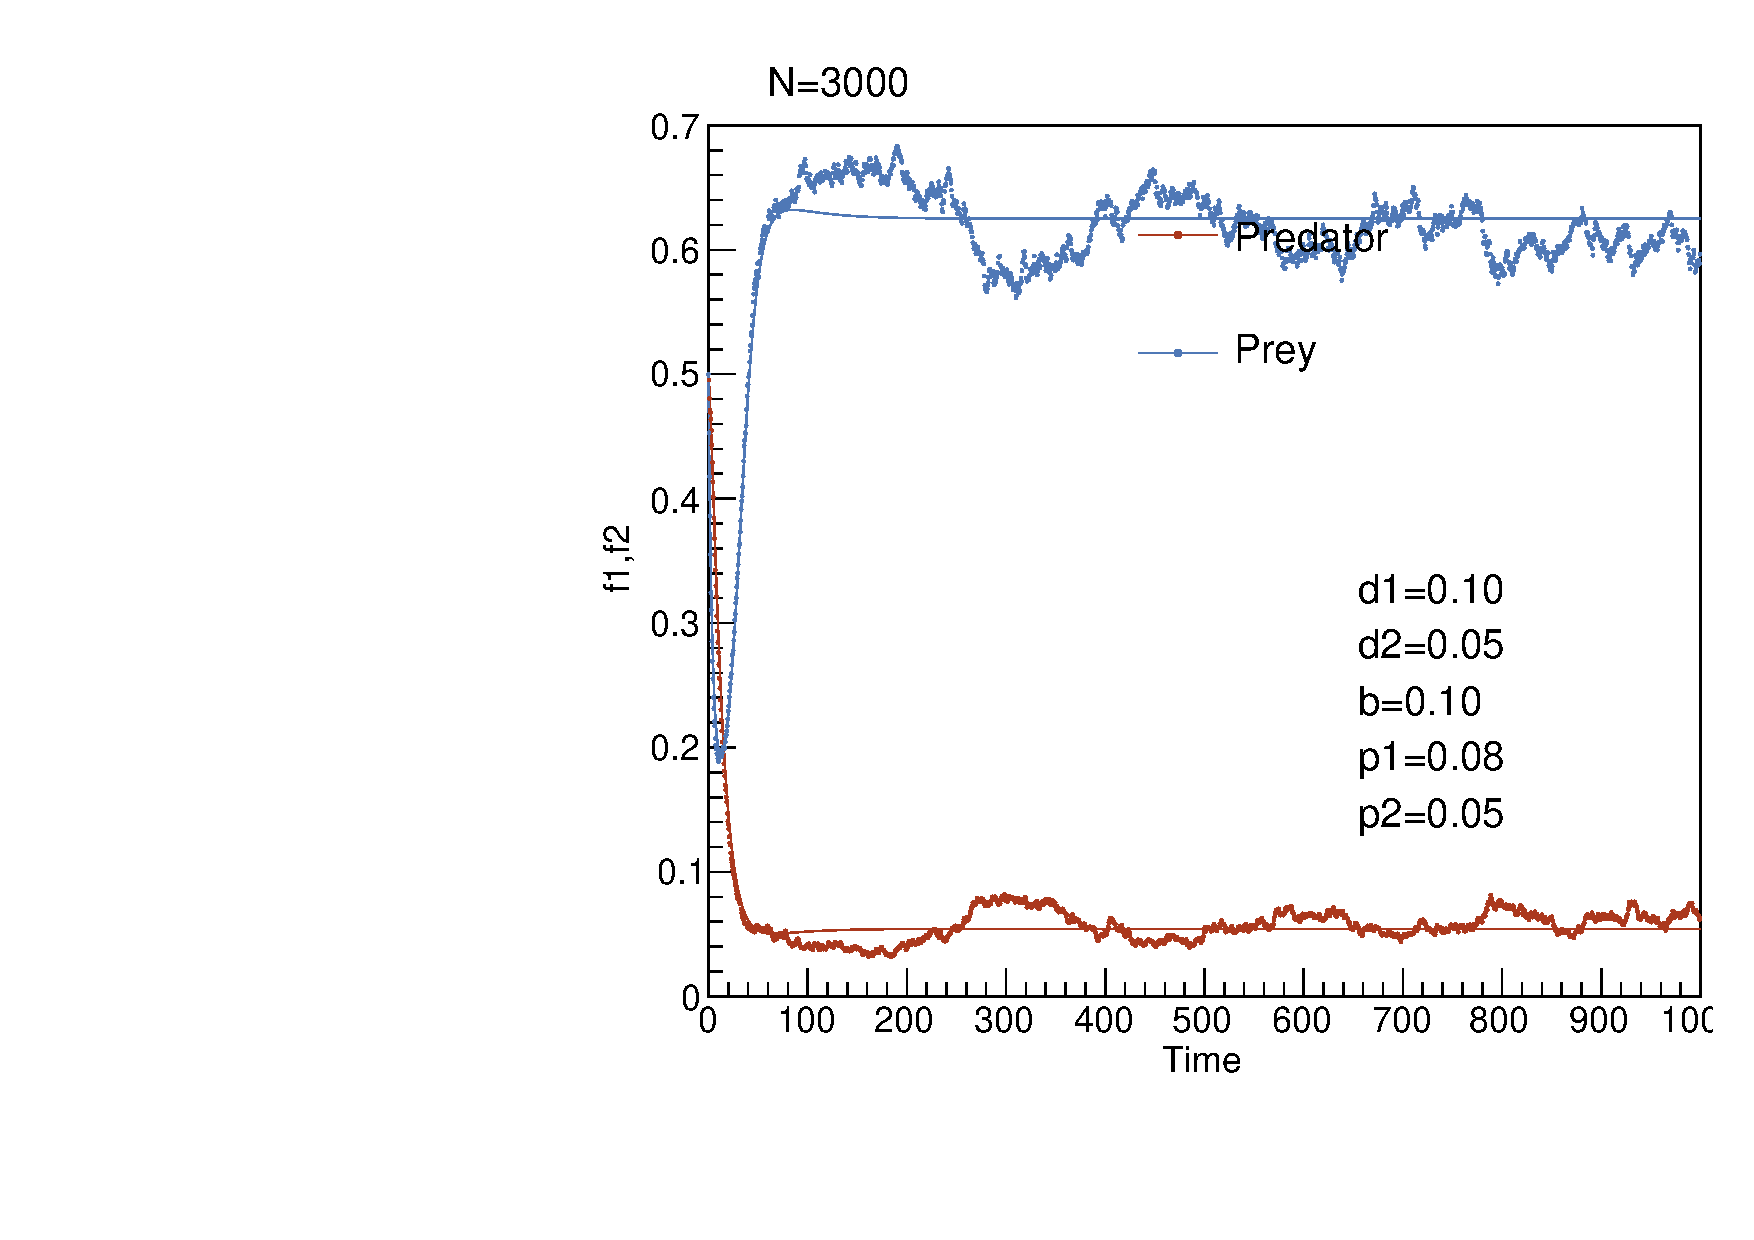
\includegraphics[width=.32\textwidth]{stochIBM_NTot3000_p10p08_20171201.pdf} 
    \caption{}
    \label{fig:fig4}
\end{figure}

In Fig.~\ref{fig:fig4} we repeat the simulations but tweak the parameter p1 to reduce the payout such that the system no longer oscillates. With this change the stochastic model no longer oscillates with a regular period or amplitude, but rather appears as fluctuations around the central, stable value predicted in the deterministic model.

\section{3.b}

\begin{figure}[H]
    \centering
    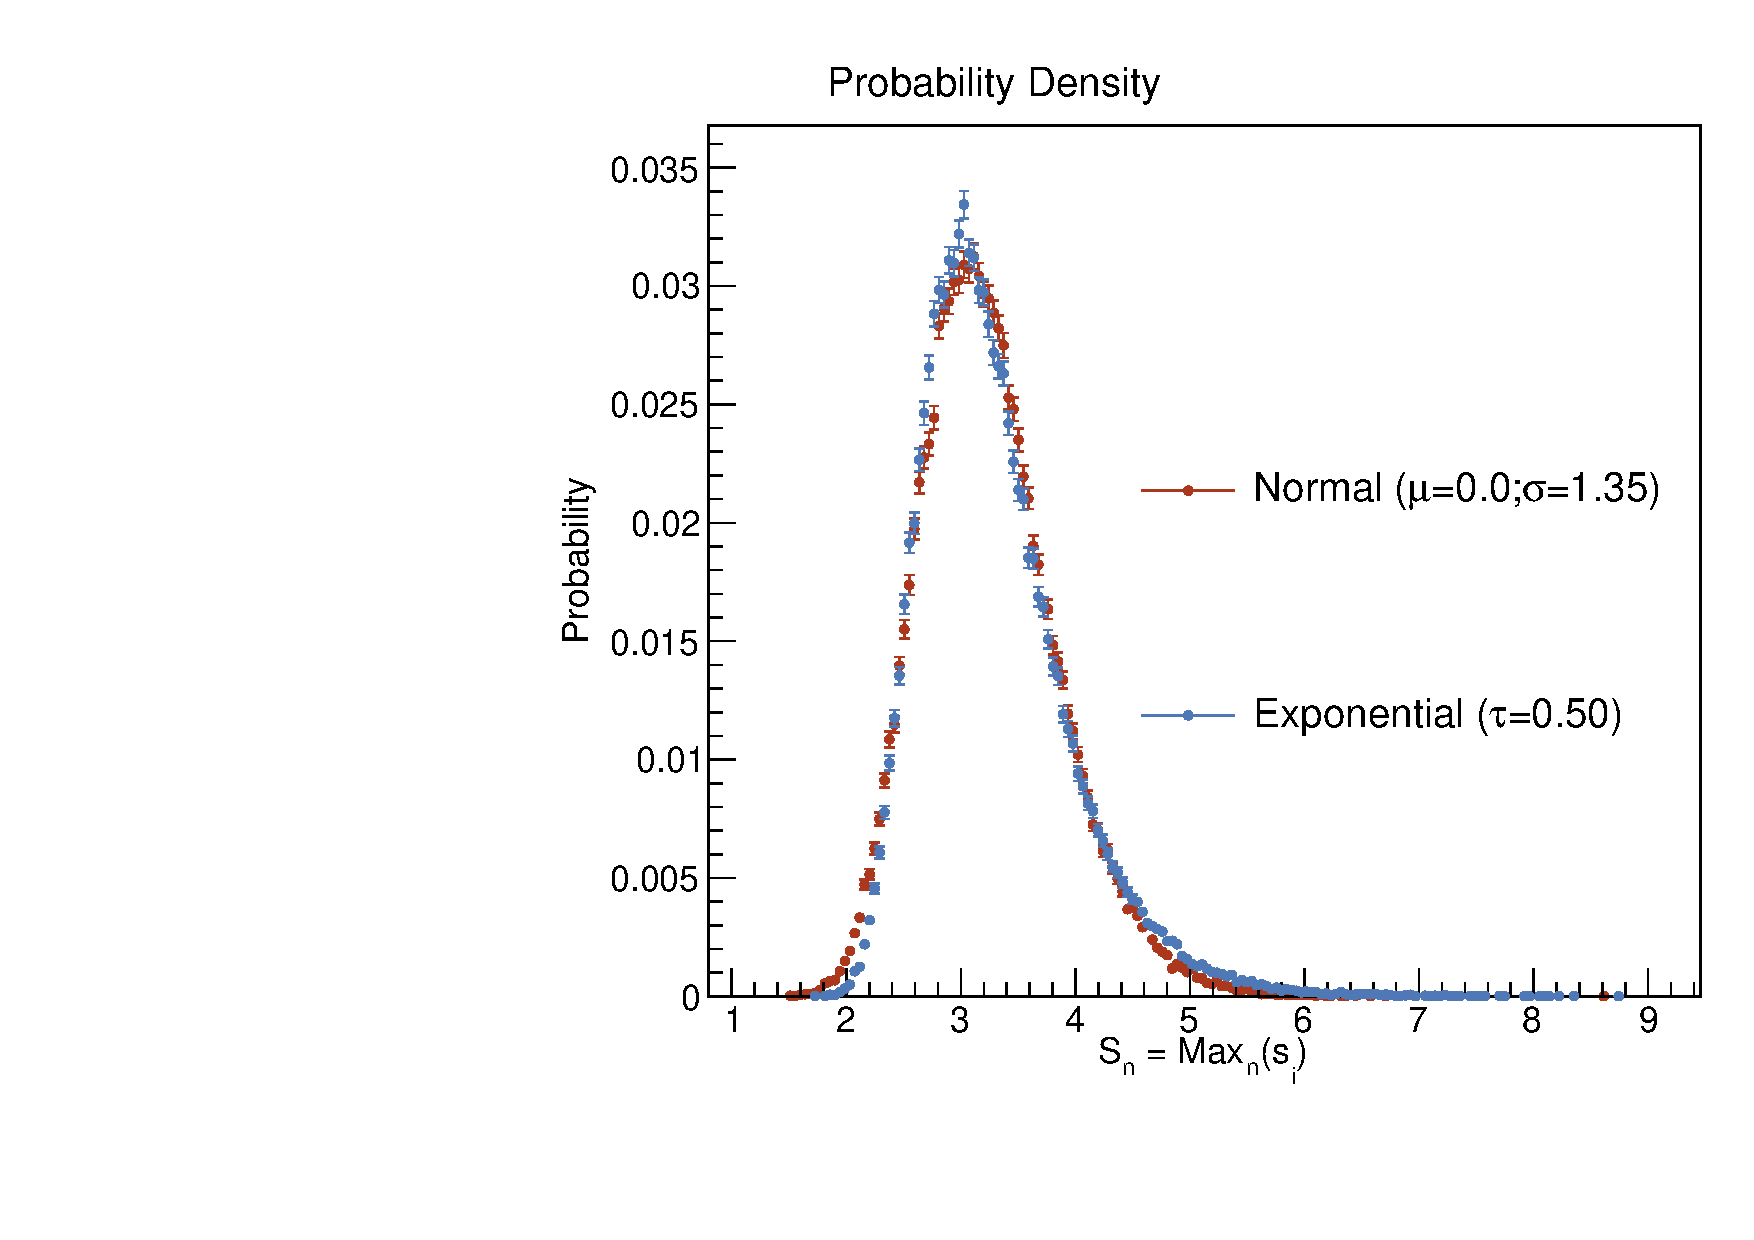
\includegraphics[width=.45\textwidth]{simulate_20171201.pdf} 
    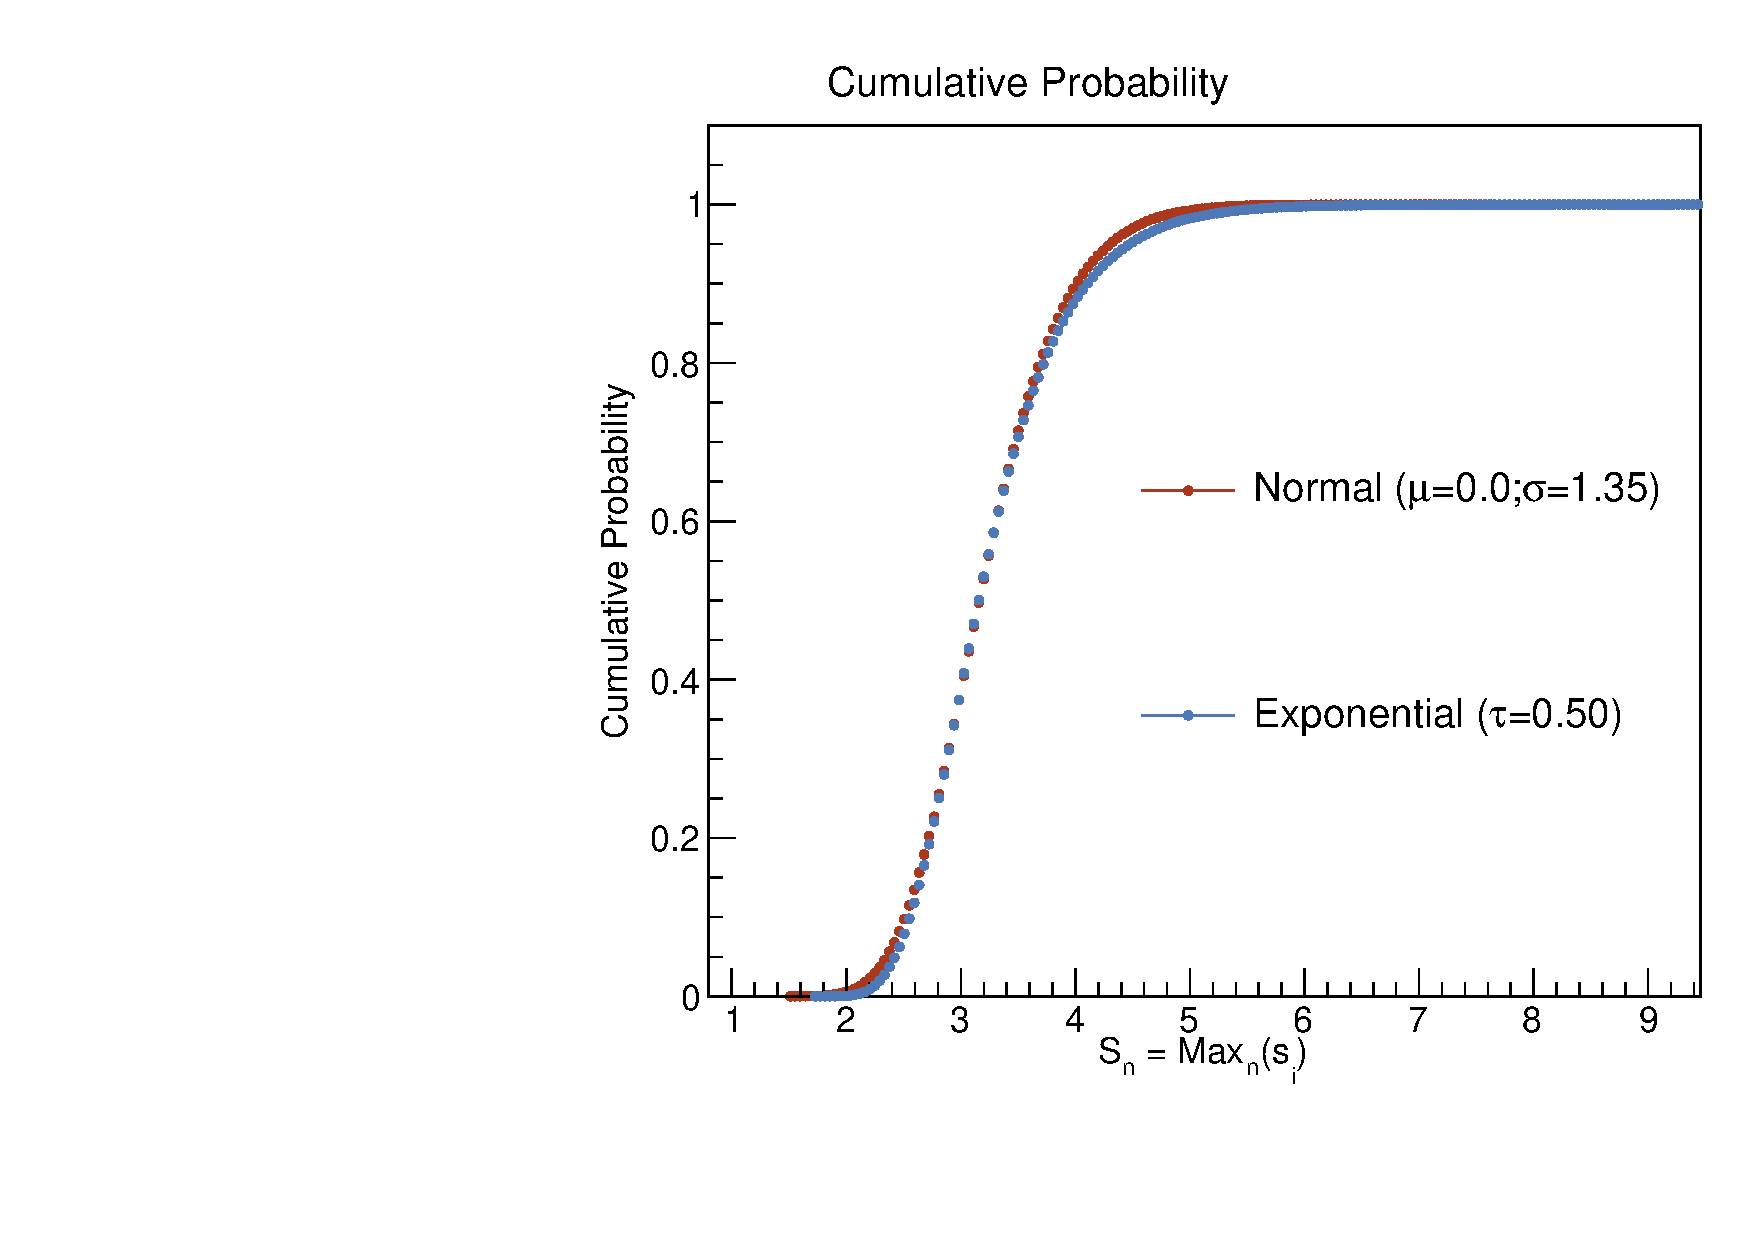
\includegraphics[width=.45\textwidth]{simulate_Cumulative_20171201.pdf} 
    \caption{}
    \label{fig:fig5}
\end{figure}

In Fig.~\ref{fig:fig5} the histogram and cumulative distribution for winning mutations is plotted for two very different underlying distributions, a gaussian and an exponential with given parametrization. The similarity and peaking behavior of the resulting final distributions shows that the combined many random variables drawn from different distributions can result in comparable final state. This makes determination of true underlying mechanism difficult, as the final state maps to many different things. In addition, given it will almost always be a cumulative distribution multiplied by the underlying density, which by definition is a finite non-zero distribution times a distribution going to zero at large values, means the probability density function will almost always peak at finite fitness.

\end{document}

